\documentclass[10pt, openany]{book}

\usepackage{fancyhdr}
\usepackage{imakeidx}

\usepackage{amsmath}
\usepackage{amsfonts}

\usepackage{geometry}
\geometry{letterpaper}

\usepackage{fancyvrb}
\usepackage{fancybox}

\usepackage{url}
\usepackage{gensymb}
\usepackage{multicol}
\usepackage{tabularx}
%
% Rules to allow import of graphics files in EPS format
%
\usepackage{graphicx}
\DeclareGraphicsExtensions{.eps}
\DeclareGraphicsRule{.eps}{eps}{.eps}{}
%
% Macro definitions
%
\newcommand{\switch}[2]{``#1''/``#2''}
\newcommand{\position}[1]{``#1''}
%
% Front Matter
%
\title{Raspberry Pi Based Mainframe Simulator}
\author{Brent Seidel \\ Phoenix, AZ}
\date{ \today }
%========================================================
%%% BEGIN DOCUMENT
\begin{document}
%
% Produce the front matter
%
\frontmatter
\maketitle
\begin{center}
This document is \copyright 2023 Brent Seidel.  All rights reserved.

\paragraph{}Note that this is a draft version and not the final version for publication.
\end{center}
\tableofcontents
\listoffigures
\listoftables

\mainmatter
%----------------------------------------------------------
\chapter{Introduction}
A rather simplistic view is that this provides a way to get a Raspberry Pi to blink some LEDs and read some switches.  However, this hardware could be modified for a number of other applications that require lots of discrete I/O, such as burglar alarms or sprinkler controls.

\section{Parts}
\subsection{3D Printing}
A fair bit of 3D printing is required, so having lots of filament is a good idea.  Labels on the panels are done by (on my printer with a 0.15mm layer height) printing 2 layers of the panel color, then 3 layers of a contrasting color for the text, and then the rest in the panel color.  The panels are printed with the text faced down.  You may wish to tinker with this for your printer.  The actual parts are:
\begin{itemize}
  \item Four or six racks depending on whether you want a 16 or 32 bit system.
  \item One processor tray.
  \item Two or three discrete I/O trays.
  \item One control panel
  \item One modes panel
  \item Two or four address/data panels (starting at 0, 8, 16, and 24).
\end{itemize}

\subsection{Electronic Parts}
Note that soldering will be required so a soldering station with appropriate tools and solder will be required in addition to the following.
\begin{itemize}
  \item One Raspberry Pi 3B computer (available from many places).
  \item At least four or up to eight MCP23017 I2C 16 bit input/output port expander chips (p/n 732 from Adafruit).
  \item One 28-pin DIP socket per MCP23017.  (eg p/n A120353-ND from Digi-Key)
  \item Recommended one LTC4311 I2C Extender/Active Terminator (p/n 4756 from Adafruit).
  \item One set of Female/Male jumper wires (p/n 1954 from Adafruit).  These are used to connect from the Raspberry Pi to the rest of the circuitry since female connectors are needed on the Raspberry Pi end).
  \item Hookup wire, preferably multi-colored (available from many places).
  \item 36 pin 0.1'' female header (5 pack p/n 598 at Adafruit).  You may need a couple packs.
  \item 23 to 39 Mini panel mount SPDT toggle switches (p/n 3221 from Adafruit).  Feel free to use other switches if you like, though you may need to adjust the hole sizes in the panels.
  \item Lots of 5mm oval LEDs (I used red, but you can use other colors) (eg p/n C5SMF-RJF-CT0W0BB1-ND from Digi-Key (buy a pack of 100 for a price discount, you can always use the excess in other projects)).
  \item Two or three IOBoard PCBs from the Circuits repository.
  \item Several 10-conductor ribbon cable breakout PCBs from the Circuits repository
  \item 4 to 6 LED PCBs from this repository.
\end{itemize}

\subsection{Mechanical Hardware}
I have a Phillips Panhead Electronic Hardware Kit from Digi-Key (p/n 1602-KIT-ND) that has an assortment of machine screws and nuts.  I used these because they were handy.

%----------------------------------------------------------
\chapter{Hardware}

\section{Electronics}
\subsection{Processor}
I had a Raspberry Pi 3 board laying around so I figured that I would use it.  Interestingly, this is a more powerful computer than many of the processors it might be used to simulate.

\subsection{Discrete I/O}
This uses the IOBoard in the Circuits repository.  Two or three of these boards will be required.  Refer to the repository for assembly details.

\section{3D Printed Parts}
\subsection{Racks}
Each rack is a bbs\_rack2(10, 6, 4).  The size is basically constrained by what my 3D printer can do.  Each of these requires about 15 hours to print on my printer.  Two of these can be bolted together side-by-side and fit in a 19 inch rack.  This is the approximate size of the classic computer equipment.  Multiple racks can be bolted together vertically as needed to provide panel space.  Each rack has slots for two vertically oriented trays.

\subsection{Processor Tray}
 The processor tray has mounting holes for the Raspberry Pi processor board. It also has a 10-conductor ribbon cable breakout board for connecting to the I2C bus ribbon cable.  Also on the tray is a LTC4311 I2C Extender/Active Terminator (p/n 4756 from Adafruit).  This may not strictly be necessary, but since the I2C bus will be running off to several other boards, I thought that it might be a good idea..

\subsection{Discrete I/O Tray}
Each of these trays has one IOBoard PCB.  These trays would typically be mounted in the slot next to the panel.  The tray has 4 10-pin connections and can interface with up to 32 GPIOs, typically 16 LEDs and 16 switches.  One additional connector is provided to connect the the power and I2C bus from the processor.

\subsection{Address/Data Panels}
The address/data panels provide 8 switches and LEDs numbered consecutively from right to left.  The starting number is selectable in the model.  Each panel has two cables (one for LEDs and one for switches) that attach to connectors on the discrete I/O boards.  Enough of these need to be provided to account for all the address and data lines in the simulated processor.  A system would typically have two or four of these panels for 16 or 32 bit systems.  Note that there are many cases where the number of address lines does not match the number of data lines.  In these cases panels would need to be provided for whichever number is greater.

\subsection{Control Panel}
At this point, without an actual CPU simulation, this is mostly a way to organize what needs to be in a relatively generic control panel.  The following functions are needed:
\begin{itemize}
  \item Read from a memory location.
  \item Write to a memory location.
  \item Stop/pause processor execution.
  \item Start processor execution at a specified address.
  \item Continue processor execution.
  \item Reset the processor.
\end{itemize}

The following switches are defined on the panel:
\begin{itemize}
  \item \switch{Run}{Pause} - The \position{Run} position allows program execution.  The \position{Pause} position temporarily suspends execution.  Moving the switch back to the \position{Run} position will continue where the program left off.
  \item \switch{Start}{Stop} - Moving the switch to the \position{Start} position loads a starting address to begin program execution.  The \position{Stop} position halts a program and a new starting address will need to be provided.
  \item \switch{Auto}{Man} - The \position{Auto} position allows for remote control of the simulator via a web interface.  The \position{Man} position disables remote control.
  \item \switch{Addr}{Data} - Selects display and entry of memory addresses or data.
  \item \position{Dep} deposits the switch value.  If the \switch{Addr}{Data} switch is in the \position{Addr} position, a memory address is loaded.  If the \switch{Addr}{Data} switch is in the \position{Data} position, the switch value is deposited in memory and the address incremented.
  \item \position{Exam} is used to examine memory at the current address.  The address is incremented each time the switch is moved to the \position{Exam} position.
  \item Spare - an empty position reserved for future expansion.
  \item \switch{Power}{Off} - This will eventually be wired up to control power to the Raspberry Pi computer.
\end{itemize}

\subsubsection{To Specify an Address}
Note that if the word size is greater than 8 bits, some of the lower order address bits may be ignored.
\begin{itemize}
  \item Toggle the desired address using the address/data switches.
  \item Move the \switch{Addr}{Data} switch to the \position{Addr} position.
  \item Move the ``Dep'' (deposit) switch to the \position{Dep} position.
  \item Once the LED for the ``Dep'' switch illuminates, move the switch to the unlabeled position.
\end{itemize}

\subsubsection{To Read Memory}
\begin{itemize}
  \item Specify the starting address as described above.
  \item Move the \switch{Addr}{Data} switch to the \position{Data} position.
  \item Move the ``Exam'' switch to the \position{Exam} position.
  \item The contents of memory at the specified address will be displayed in the Address/Data LEDs.
  \item The \switch{Addr}{Data}  switch can be used to toggle between display of the address and the data.
  \item Move the ``Exam'' switch to the unlabeled position.  This increments the internal address pointer so that by toggling this switch a block of memory can be modified.
\end{itemize}

\subsubsection{To Write Memory}
\begin{itemize}
  \item Specify the starting address as described above.
  \item Move the \switch{Addr}{Data}  switch to the \position{Data} position.
  \item Toggle the desired data using the address/data switches.
  \item Move the ``Dep'' switch to the \position{Dep} position.
  \item The contents of memory at the specified address will be updated and displayed in the Address/Data LEDs.
  \item The \switch{Addr}{Data} switch can be used to toggle between display of the address and the data.
  \item Move the ``Dep'' switch to the unlabeled position.  This increments the internal address pointer so that by toggling this switch a block of memory can be examined.
\end{itemize}

\subsubsection{To Start Execution at a Specific Address}
\begin{itemize}
  \item Move the \switch{Start}{Stop} switch to the \position{Stop} position.
  \item Move the \switch{Addr}{Data} switch to the \position{Addr} position.
  \item Toggle the address using the address/data switches.
  \item Move the \switch{Start}{Stop} switch to the \position{Start} position.
  \item If the \switch{Run}{Pause} switch is in the \position{Pause} position, move it to the \position{Run} position.
\end{itemize}

\subsection{Mode Panel}
This is a display only panel to show the processor and memory access modes.  It has seven labeled positions in two groups separated by a spare.  The first group is the processor mode.  This indicates which of four possible modes (User, Supervisor, Executive, or Kernel) the processor is in.  The second group indicates the type of memory access.  There are four possibilities: Instruction (read-only), Data (read/write), I/O (read/write), and Interrupt (read-only).

\section{Assembly}

\subsection{Planning}
The first decision is if you want to simulate a 16 bit or 32 bit (or something else) system.  Each panel can hold up to 8 LEDs and switches.  Each MCP23017 can control 16 LEDs or switches, so 2 MCP23017s can control 2 panels.  Each rack has space for 1 panel and two circuit trays.  If you attach two racks side by side, they will approximately fit in a 19 inch rack (as I don't have a standard 19 inch rack, you will probably have to design and print some sort of adapter).

Once you've decided on your system size, then you need to figure out how to arrange things.  See Table \ref{tbl:Basic} for an example arrangement.  Once this is finished, then you can go ahead and figure out how long your cables need to be.

\begin{table}[ht!]
  \caption{Example 16 Bit Processor Layout}
  \label{tbl:Basic}
  \centering
  \begin{tabular}{|l|l|}
    \hline
    Processor & empty\\
    Address Data Panel Controller & empty\\
    Address/Data 8-15 Panel & Address/Data 0-7 Panel\\
    \hline
    empty & empty\\
    Control Panel Controller & empty\\
    Mode Panel & Control Panel\\
    \hline
  \end{tabular}
\end{table}

\subsection{Processor Tray}
The processor is an already assembled Raspberry Pi.  I've used a Pi 3B, but others should work as long as they have the same pinout and hole pattern.  What needs to be assembled is the connection from the Pi to the bus.  This starts with the bare breakout board in Figure \ref{fig:BreakoutBare}.  A connector needs to be added as shown in Figure \ref{fig:BreakoutConnector}.  Finally, a female header and jumper wire needs to be added to connect to the Raspberry Pi and make sure that both of the ground conductors are connected to ground as shown in Figure \ref{fig:BreakoutJumper}.

\begin{figure}[ht!]
  \centering
  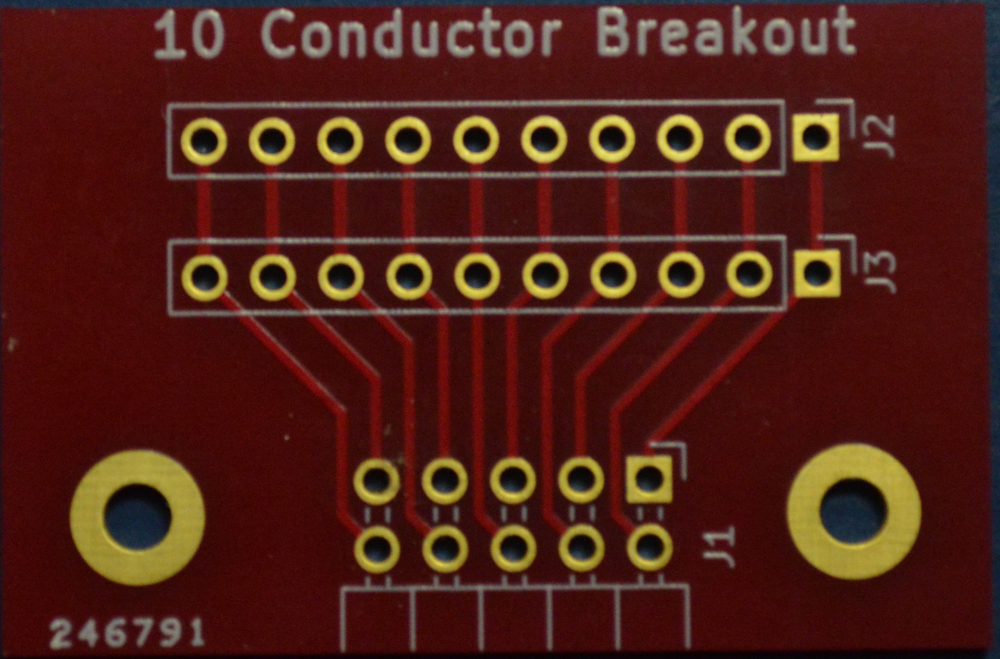
\includegraphics[width=0.9\textwidth]{../Pict/Breakout-Bare.jpg}
  \caption{Bare Breakout Board}
  \label{fig:BreakoutBare}
\end{figure}

\begin{figure}[ht!]
  \centering
  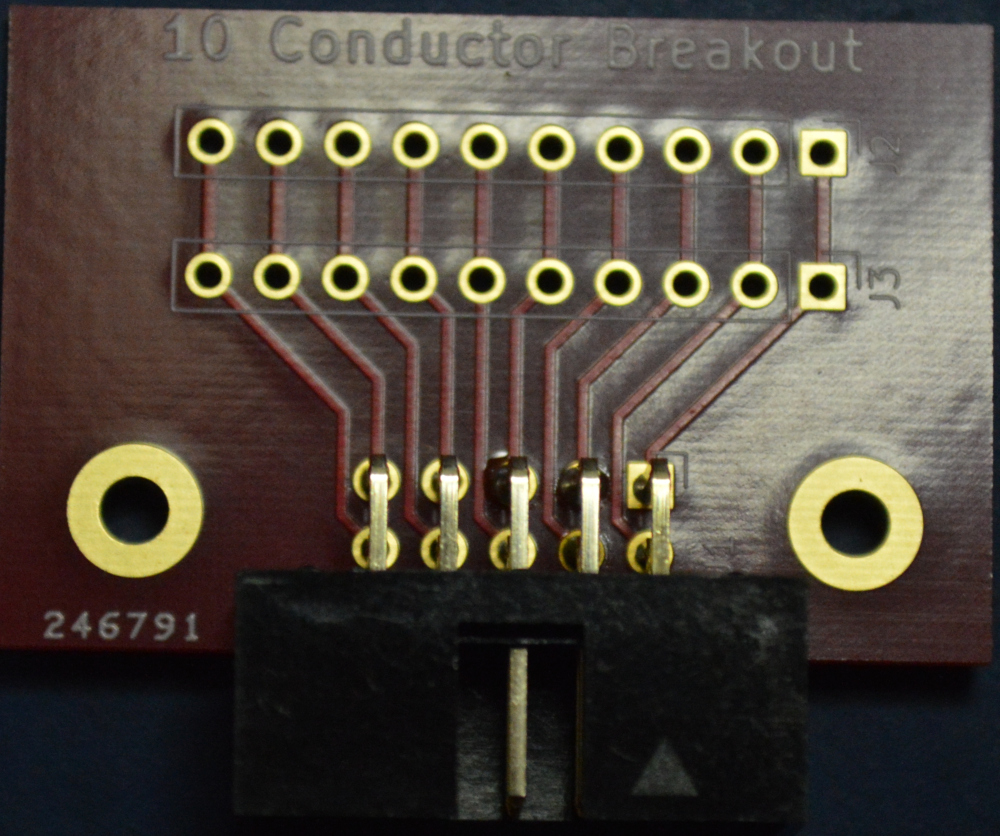
\includegraphics[width=0.9\textwidth]{../Pict/Breakout-Connector.jpg}
  \caption{Breakout Board with Connector}
  \label{fig:BreakoutConnector}
\end{figure}

\begin{figure}[ht!]
  \centering
  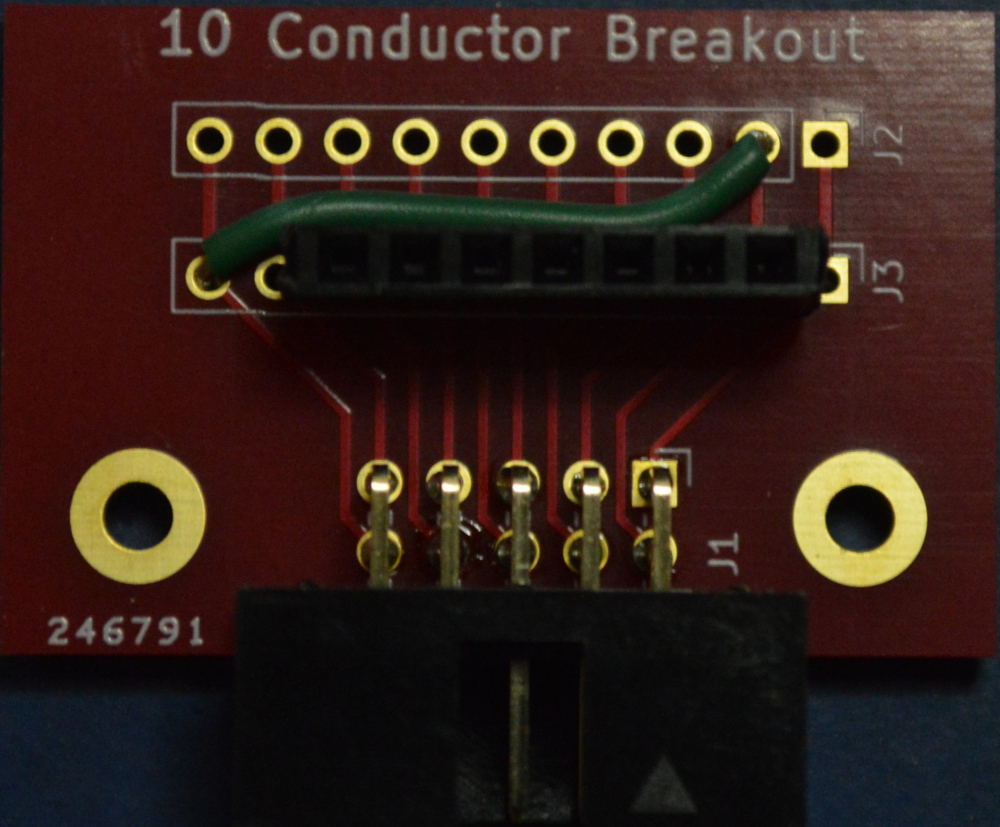
\includegraphics[width=0.9\textwidth]{../Pict/Breakout-Jumper.jpg}
  \caption{Breakout Board with Connectors and Jumper}
  \label{fig:BreakoutJumper}
\end{figure}

\subsubsection{Optional Active Terminator}
Adafruit sells an active I2C terminator that you can connect to the I2C bus to improve the signal quality.  This is optional, but you may wish to consider this if the bus doesn't work properly.  It is soldered to the breakout board by fairly short wires as in Figure \ref{fig:BreakoutDriver}.  The stiffness of these wires should be adequate unless you are expecting high vibrations.  In that case, add mounting holes to the tray so that it can be screwed down.

\begin{figure}[ht!]
  \centering
  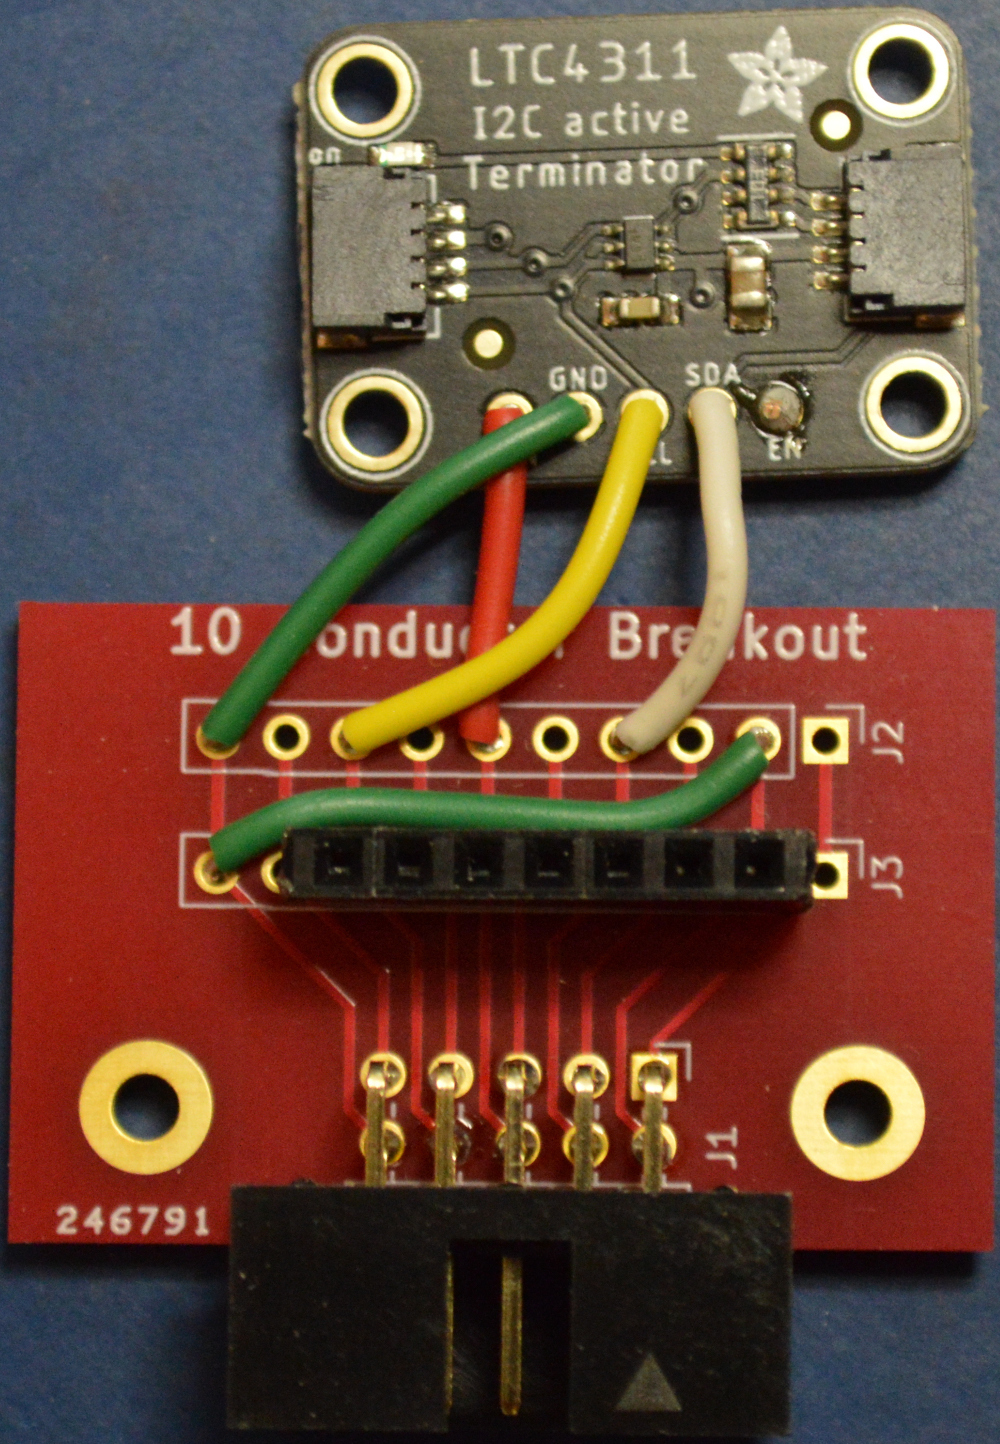
\includegraphics[width=0.9\textwidth]{../Pict/Breakout-Driver.jpg}
  \caption{Breakout Board with Active I2C Terminator}
  \label{fig:BreakoutDriver}
\end{figure}

The one fiddly bit is that a pull-up jumper needs to be added from the Active Terminator's enable pin as show in figure \ref{fig:DriverJumper}.

\begin{figure}[ht!]
  \centering
  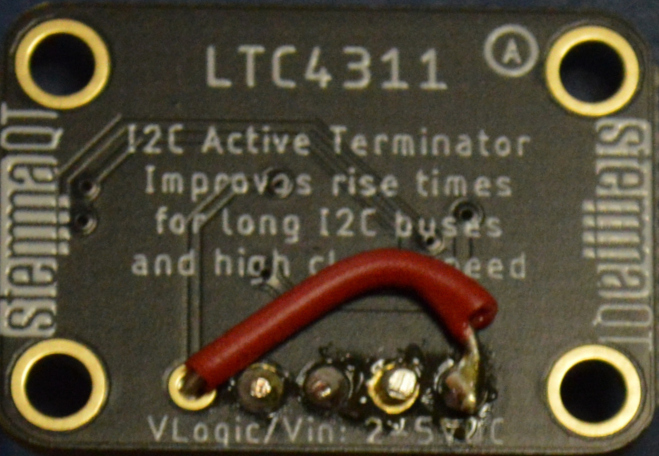
\includegraphics[width=0.9\textwidth]{../Pict/Driver-Jumper.jpg}
  \caption{I2C Active Terminator Showing Pull-Up Jumper to Enable}
  \label{fig:DriverJumper}
\end{figure}

Once the breakout board is assembled, attach it and the Raspberry Pi to the processor tray and add jumper wires from the Pi to the breakout board, as shown in Figure \ref{fig:CPUTray}.

\begin{figure}[ht!]
  \centering
  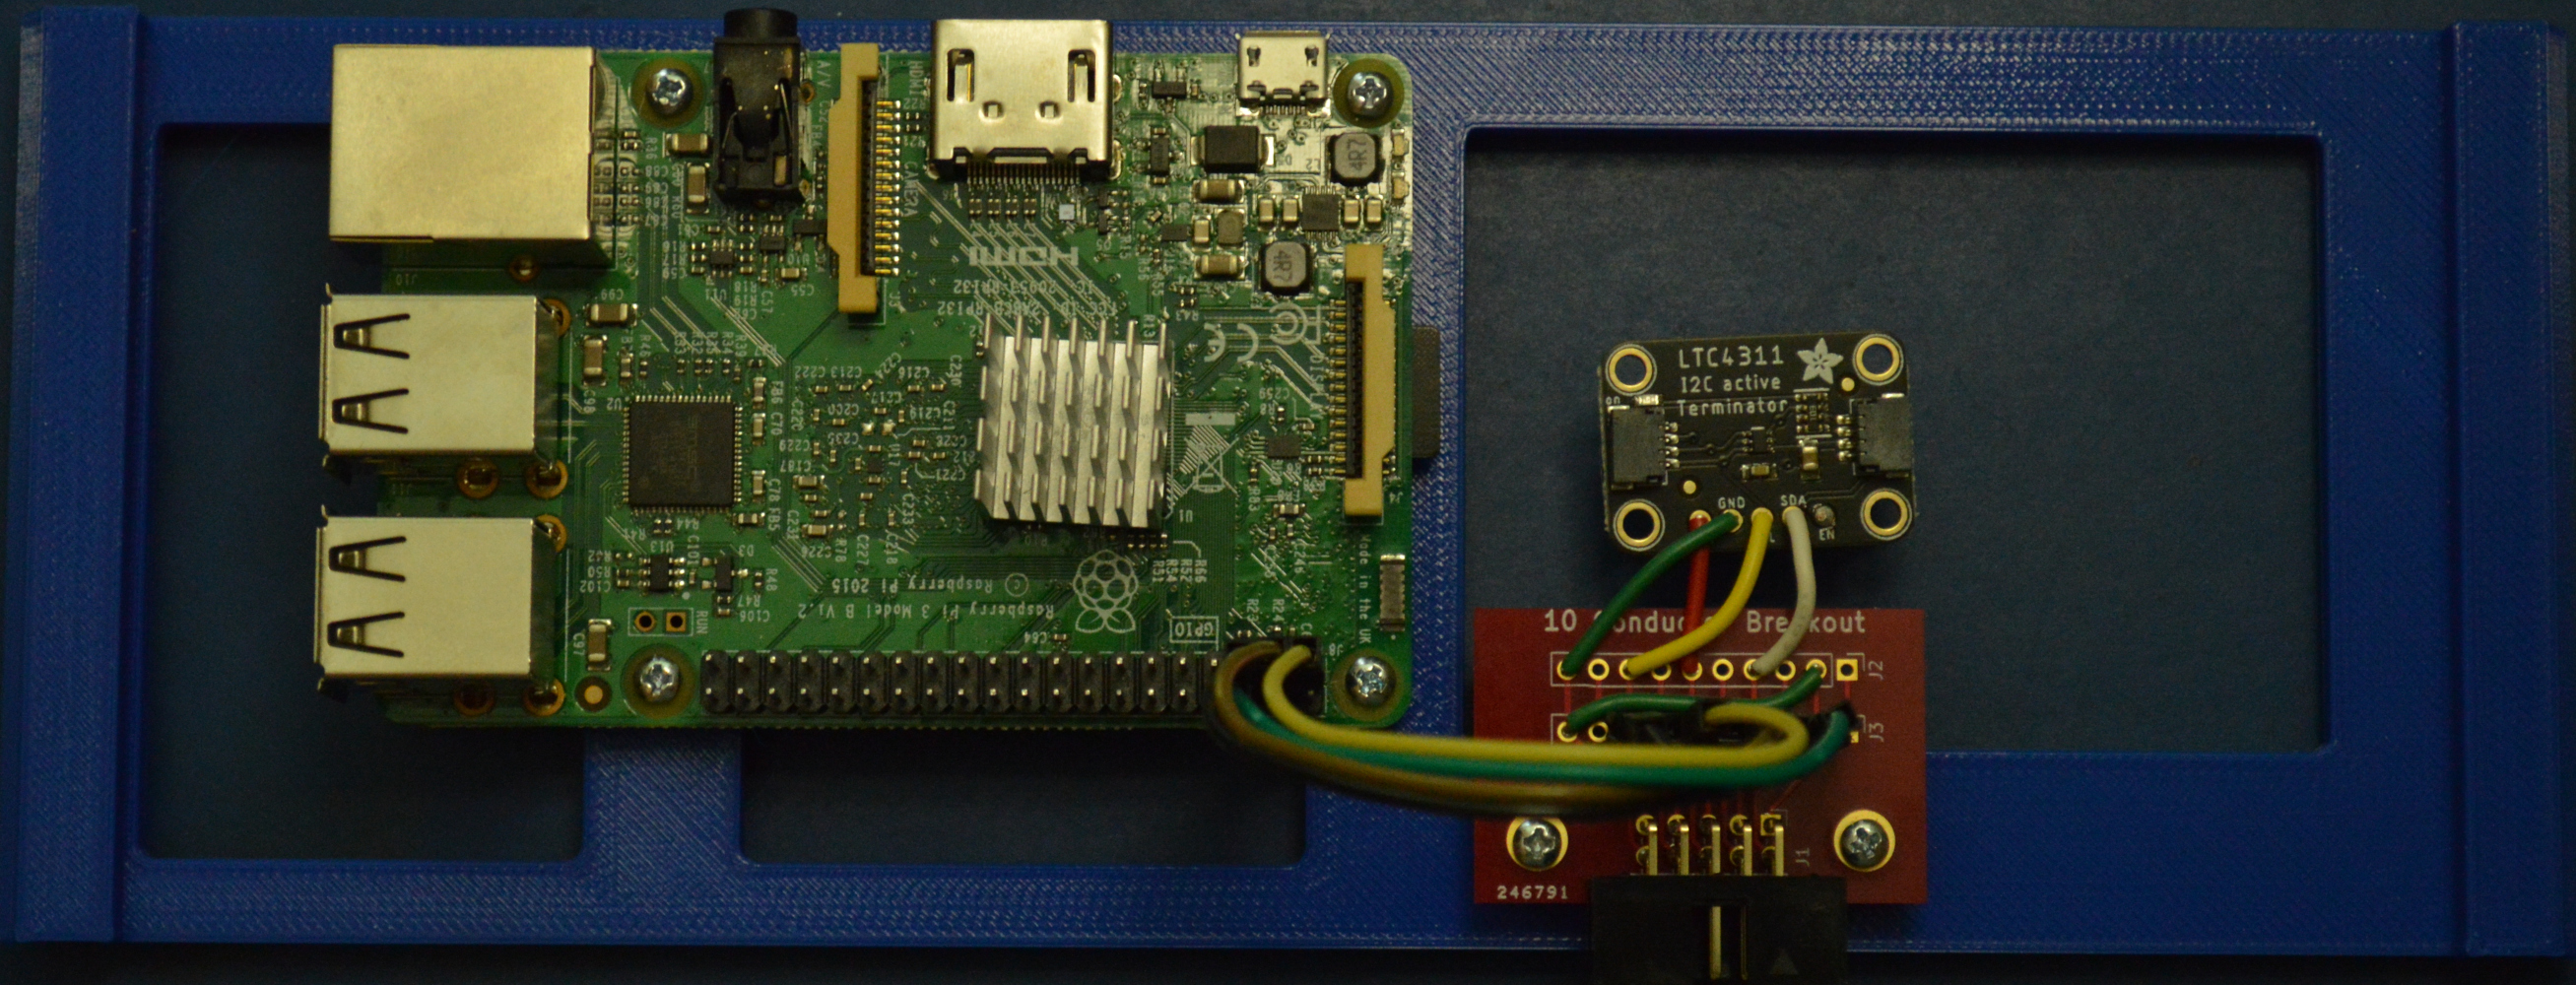
\includegraphics[width=0.9\textwidth]{../Pict/CPU-Board.jpg}
  \caption{Assembled CPU Tray}
  \label{fig:CPUTray}
\end{figure}

\clearpage
\subsection{Panel I/O Tray}
The Panel I/O Tray holds one Discrete I/O Board.  The discrete I/O boards offer 32 bits of GPIO.  Each can be configured as an input or an output.  Assembly instructions for this board are provided in the Circuits repository along with the schematics and PCB layout.

Since the power LED is meant to be on whenever power is applied, a modification needs to be made to the discrete I/O board for the mode and control panels.  This means that the SMD resistor for the power LED needs to be mounted so that it doesn't connect to the MCP23017.  It instead needs a jumper from power connected to it as shown in Figure \ref{fig:GPIOCtrl}.

\begin{figure}[ht!]
  \centering
  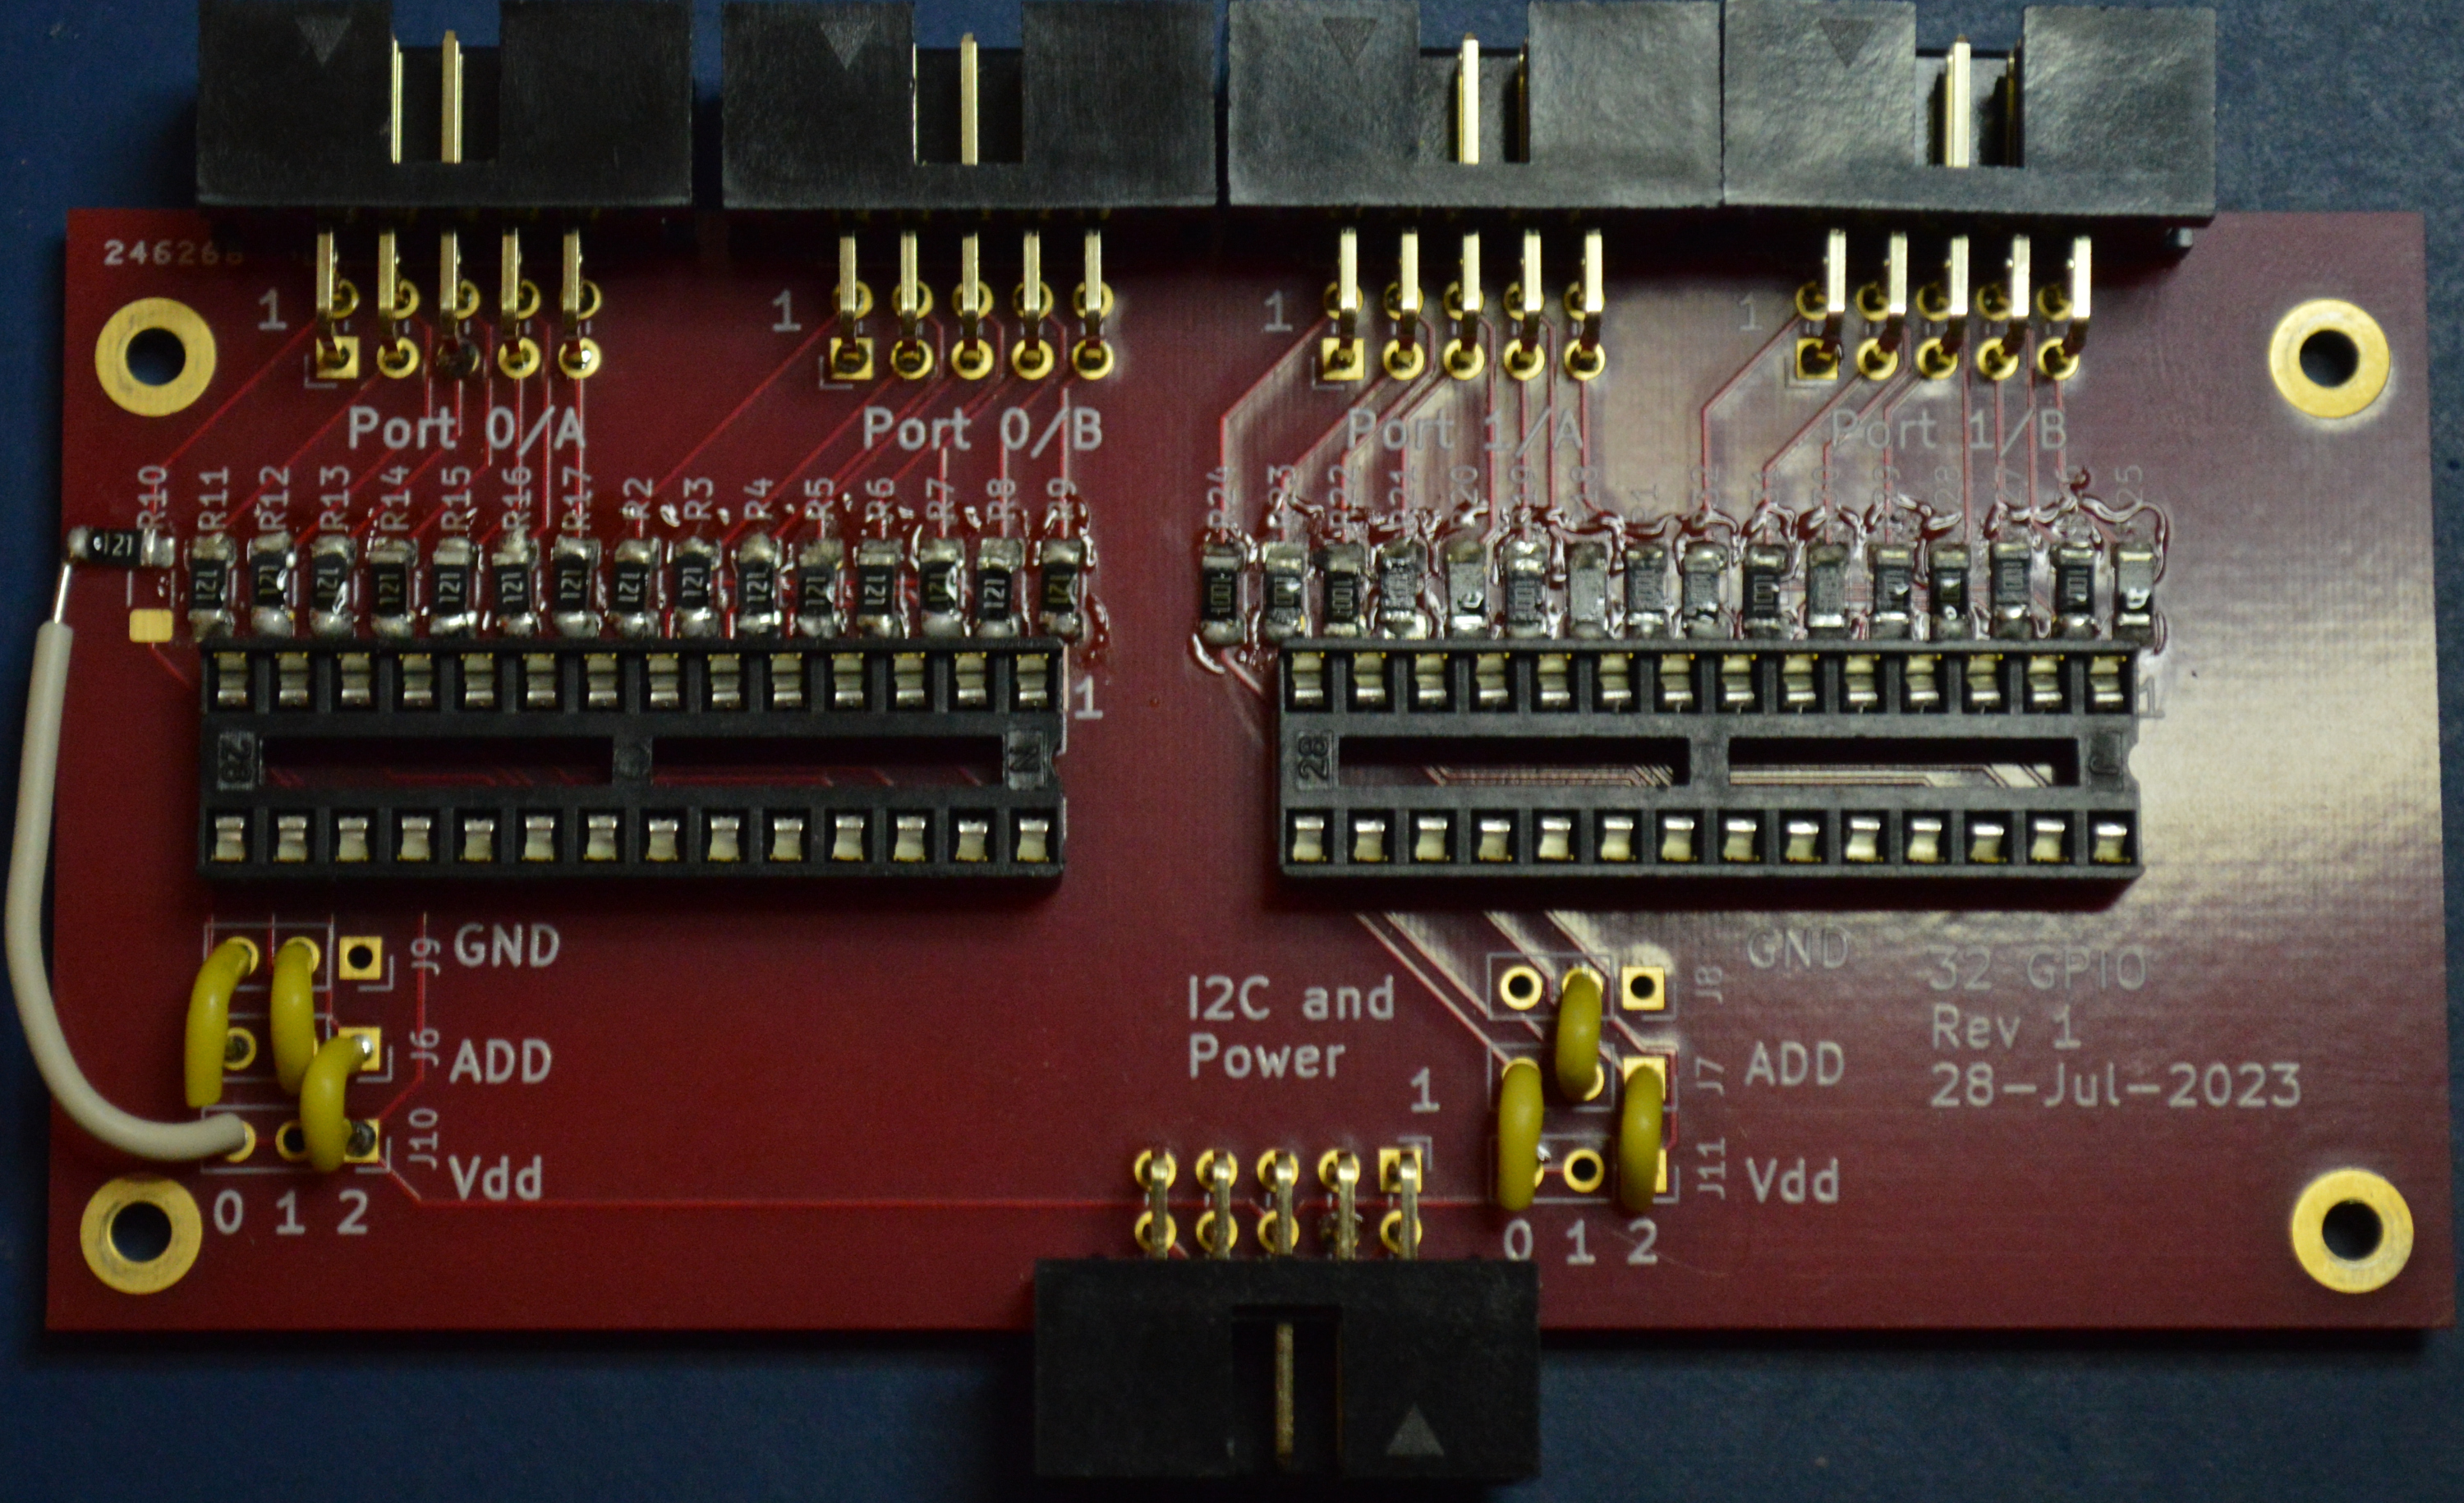
\includegraphics[width=0.9\textwidth]{../Pict/GPIO-Control.jpg}
  \caption{GPIO Board for Mode and Control Panel.  Note jumper to SMD resistor on top left for power indication.}
  \label{fig:GPIOCtrl}
\end{figure}

The I2C addresses and connectors used are in Table \ref{tbl:i2c}.

\begin{table}
  \caption{I2C Addresses for Discrete I/O Boards}
  \label{tbl:i2c}
  \centering
  \begin{tabular}{|l|l|}
    \hline
    Address & Use\\
    0 & Least significant LEDs (port A = bits 7-0, port B = bits 15-8)\\
    1 & Least significant switches (port A = bits 7-0, port B = bits 15-8)\\
    2 & Most significant LEDs (port A = bits 23-16, port B = bits 31-24)\\
    3 & Most significant switches (port A = bits 23-16, port B = bits 31-24)\\
    4 & Mode/Control LEDs (port A = control, port B = mode)\\
    5 & Control switches (port A = control, port B = unused)\\
    6 & Spare for future expansion\\
    7 & Spare for future expansion\\
    \hline
  \end{tabular}
\end{table}

\subsection{Panel LEDs}
\label{subsec:PanelLED}
The LED PCB is shown in Figure \ref{fig:LEDPCB}.  The connector is installed on the opposite side of the board from the LEDs as shown in Figure \ref{fig:LEDConnector}.  This is due to space constraints.  The LEDs are installed as shown in Figure \ref{fig:LEDLED}.  Note that the short leg of the LED goes to ground.  Once the connector is soldered, the LEDs can be inserted and hooked up to an I/O board for testing prior to soldering the LEDs.  The final assembled board after trimming the LED legs is shown in Figure \ref{fig:LEDFinal}.

\begin{figure}[ht!]
  \centering
  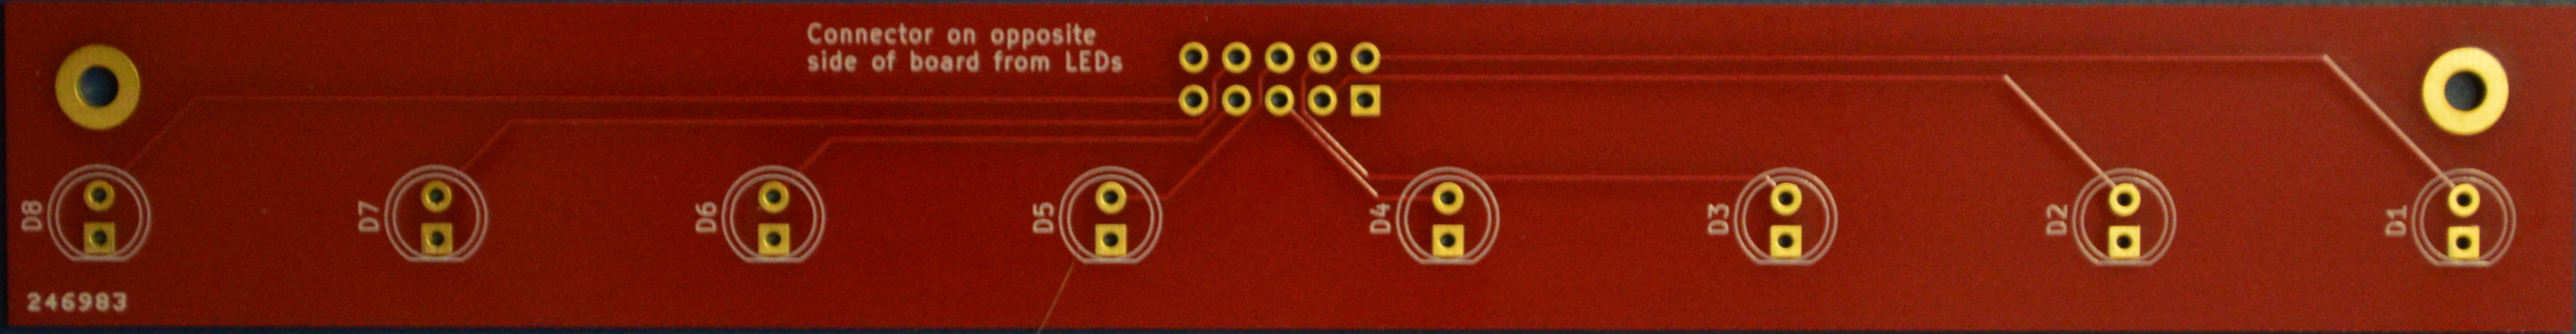
\includegraphics[width=0.9\textwidth]{../Pict/LED-Board.jpg}
  \caption{PCB for LEDs}
  \label{fig:LEDPCB}
\end{figure}

\begin{figure}[ht!]
  \centering
  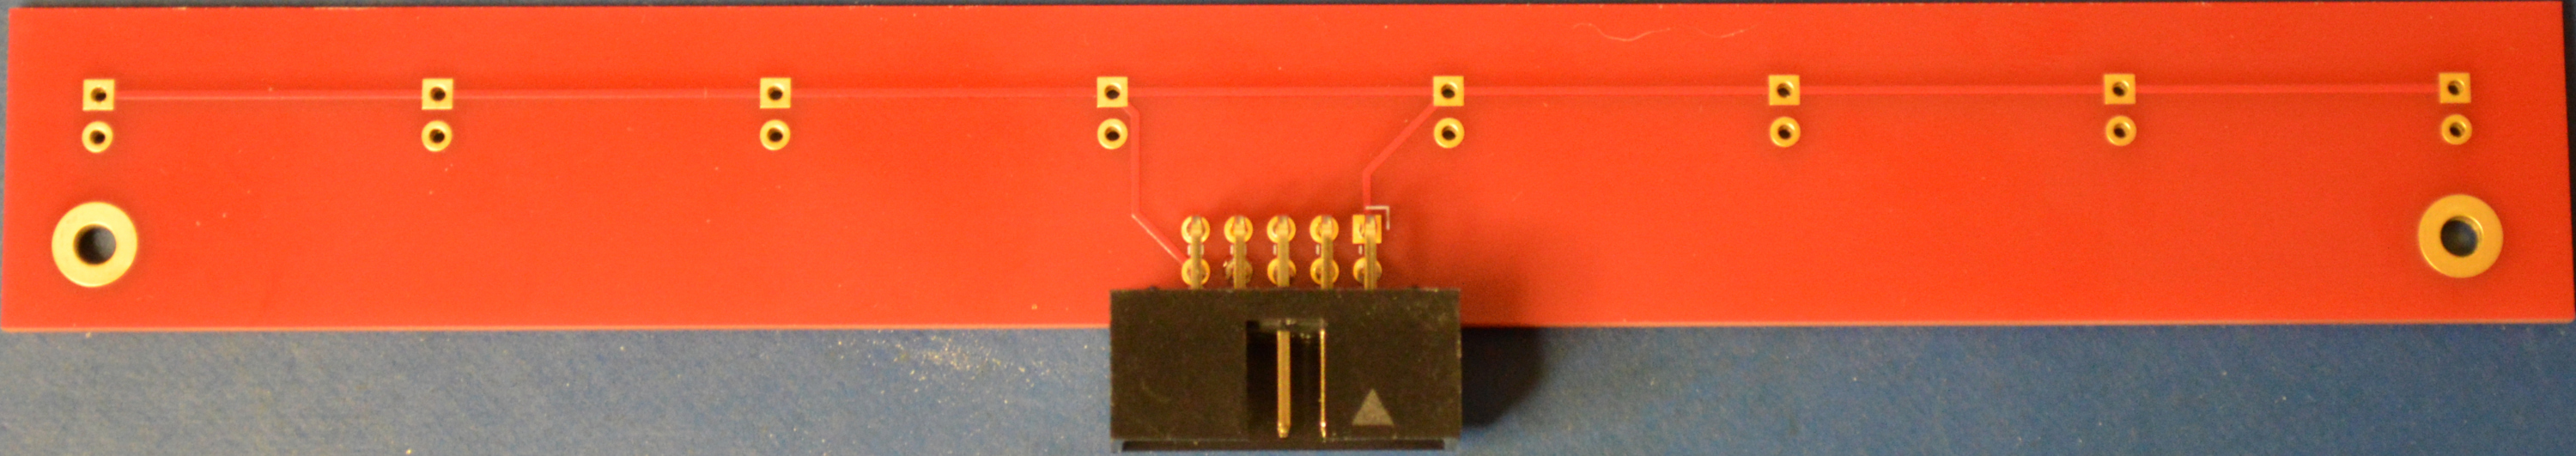
\includegraphics[width=0.9\textwidth]{../Pict/LED-Connector.jpg}
  \caption{LED PCB With Connector Installed}
  \label{fig:LEDConnector}
\end{figure}

\begin{figure}[ht!]
  \centering
  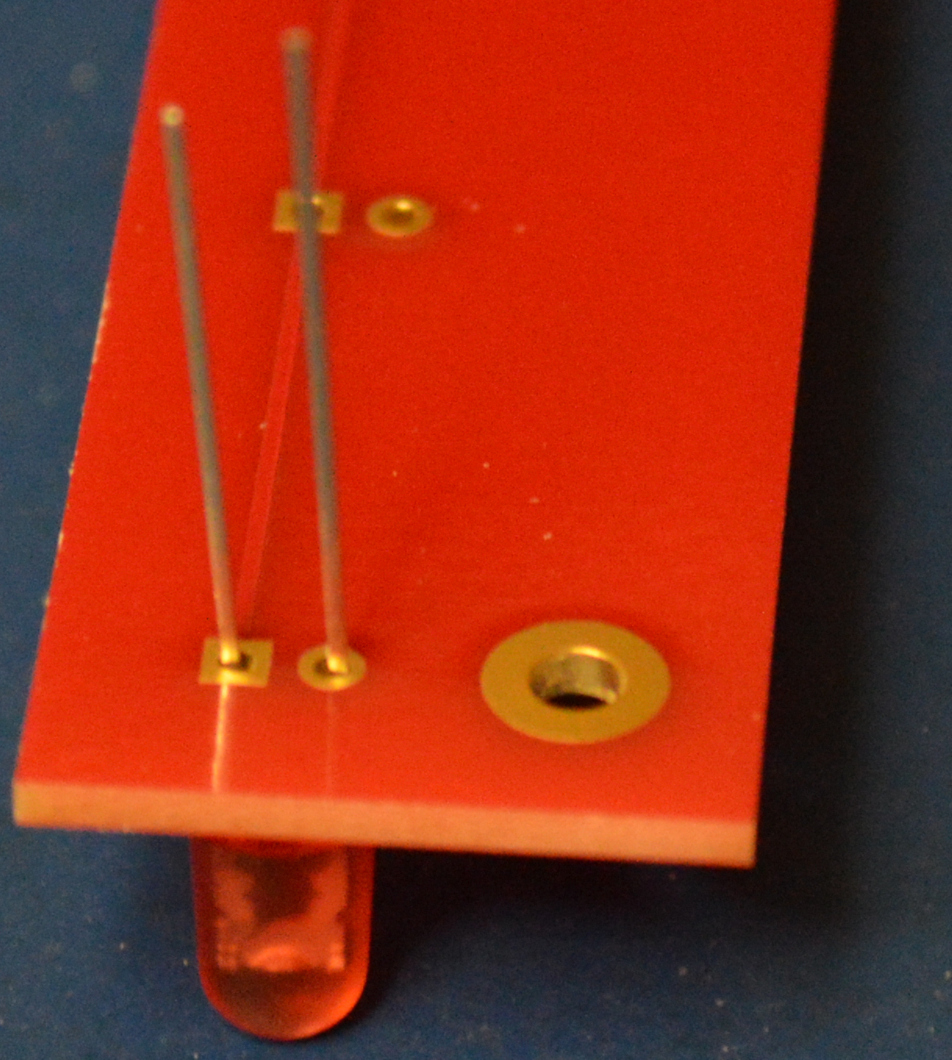
\includegraphics[width=0.9\textwidth]{../Pict/LED-LED.jpg}
  \caption{Installing LEDs in the LED PCB}
  \label{fig:LEDLED}
\end{figure}

\begin{figure}[ht!]
  \centering
  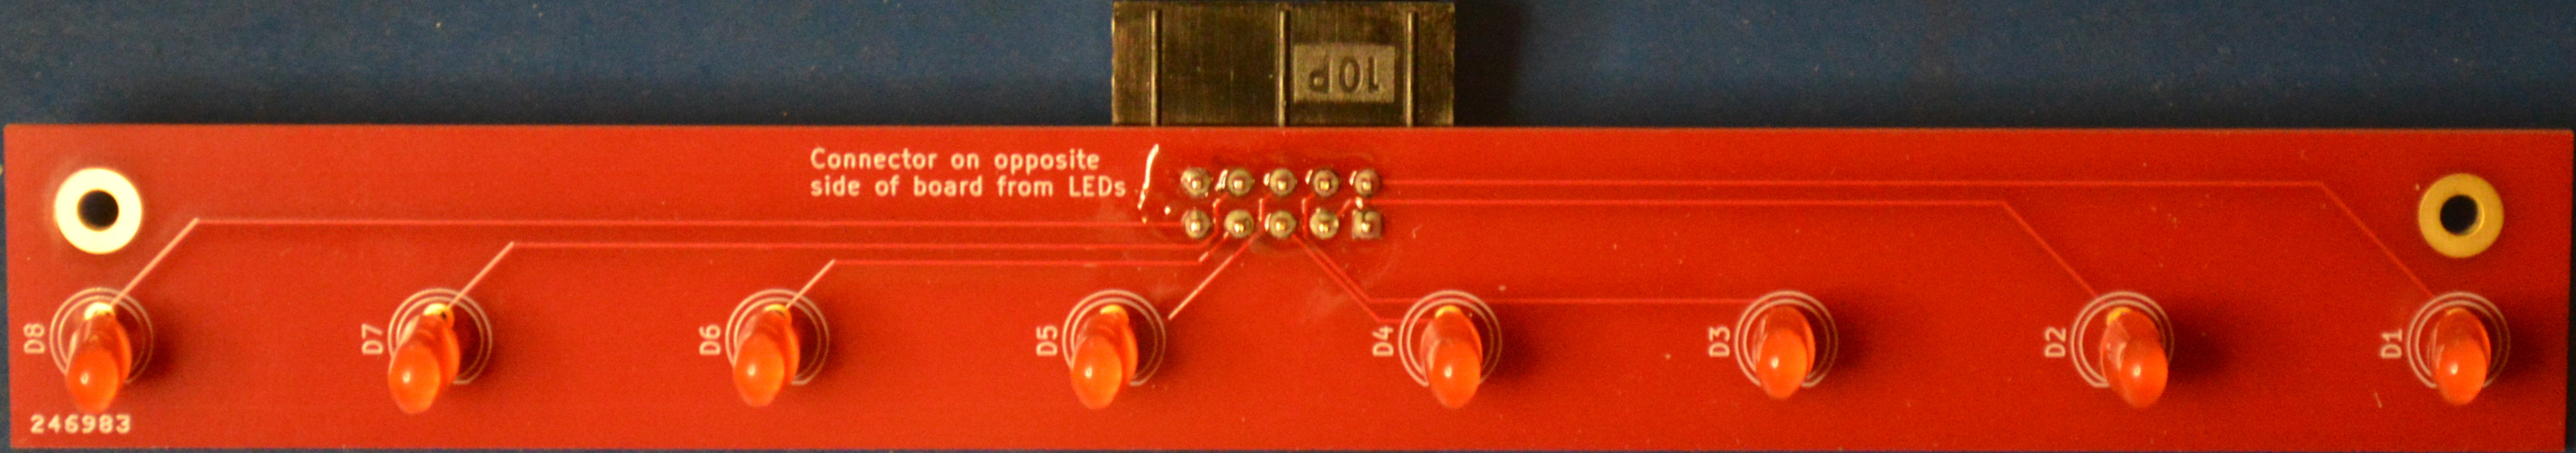
\includegraphics[width=0.9\textwidth]{../Pict/LED-Final.jpg}
  \caption{Completed LED PCB}
  \label{fig:LEDFinal}
\end{figure}

Once the LED PCB is assembled, it is be installed in a panel.  Depending on how accurate the soldering is, some adjustment may need to be done to get the LEDs to go into the holes in the panel.  Once they go, the bottom side of the PCB should be snapped into the groove in the support and screws placed in the top corners.  See Figures \ref{fig:PanelFront} and \ref{fig:PanelBack} for front and back views.

\begin{figure}[ht!]
  \centering
  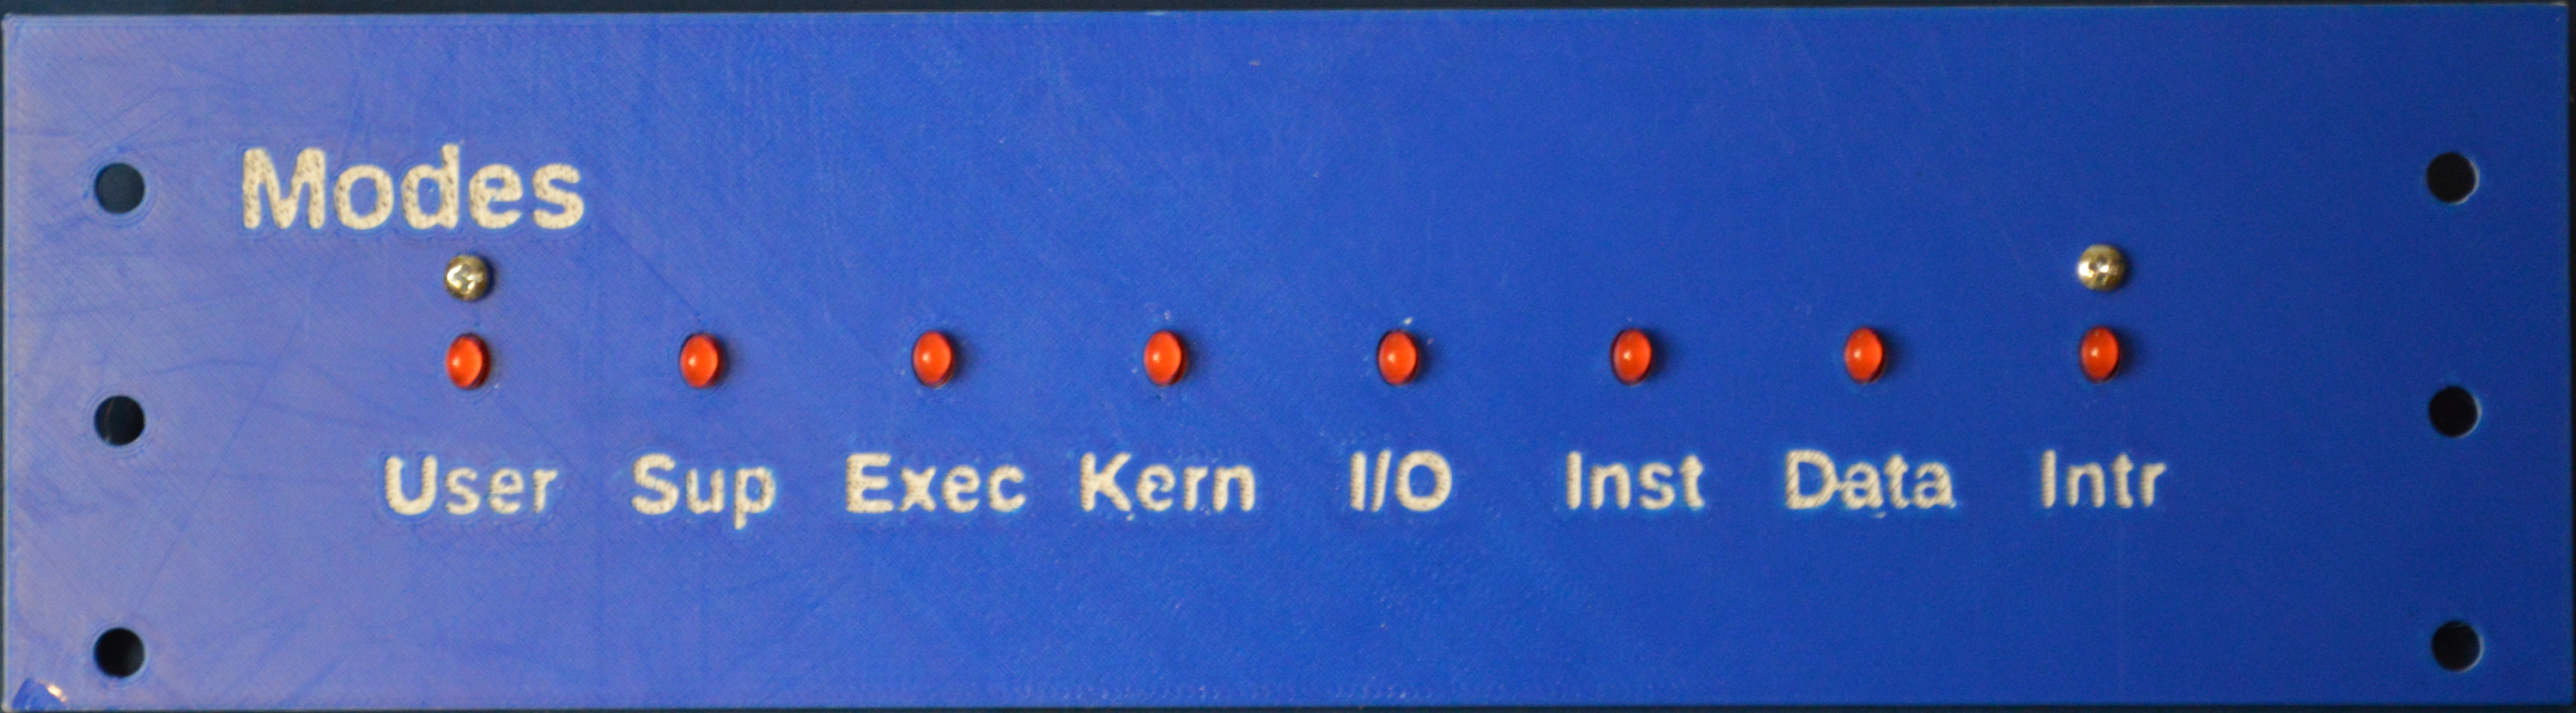
\includegraphics[width=0.9\textwidth]{../Pict/Panel-Front.jpg}
  \caption{Front of Panel with LEDs Installed}
  \label{fig:PanelFront}
\end{figure}

\begin{figure}[ht!]
  \centering
  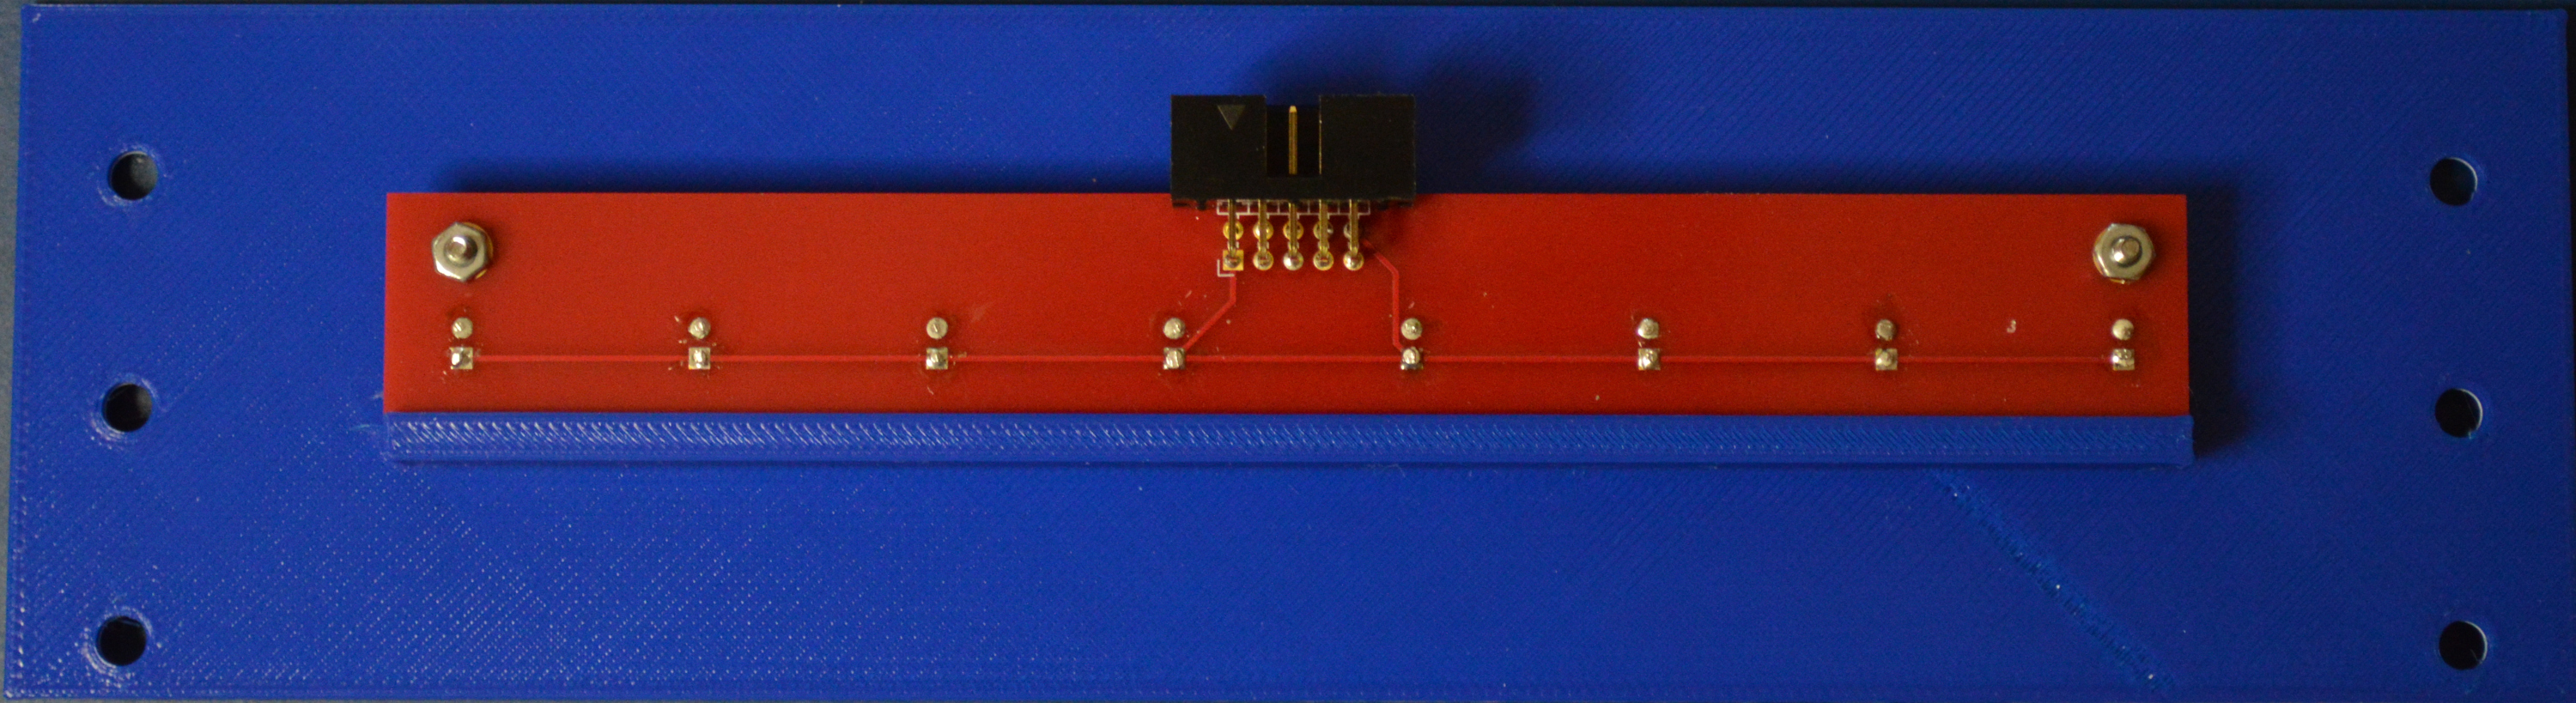
\includegraphics[width=0.9\textwidth]{../Pict/Panel-Back.jpg}
  \caption{Back of Panel with LED PCB Installed}
  \label{fig:PanelBack}
\end{figure}

\clearpage
\subsection{Panel Switches}
My implementation uses SPST switches where the center connector is common.  When the switch is in the up position, the center and lower connector are connected.  When the switch is in the down position, the center and upper connector are connected.  The MCP23017s have an optional pull-up for each input, thus the switches can be used in an open-ground configuration.  The top connectors are tied together and connected to ground.  The center connectors are connected to the individual input pins.
\begin{itemize}
  \item Install the switches as shown in Figure \ref{fig:SwitchInstalled}.
  \item Install the wiring for the switches as shown in Figure \ref{fig:SwitchWired}.  The wiring is shown going to a breakout board.  This allows a ribbon cable to be used to connect to the I/O board.  Alternating blue and white wires are used to make it a little easier to follow.  The ground wire from the breakout board is green on the far right.
\end{itemize}

\begin{figure}[ht!]
  \centering
  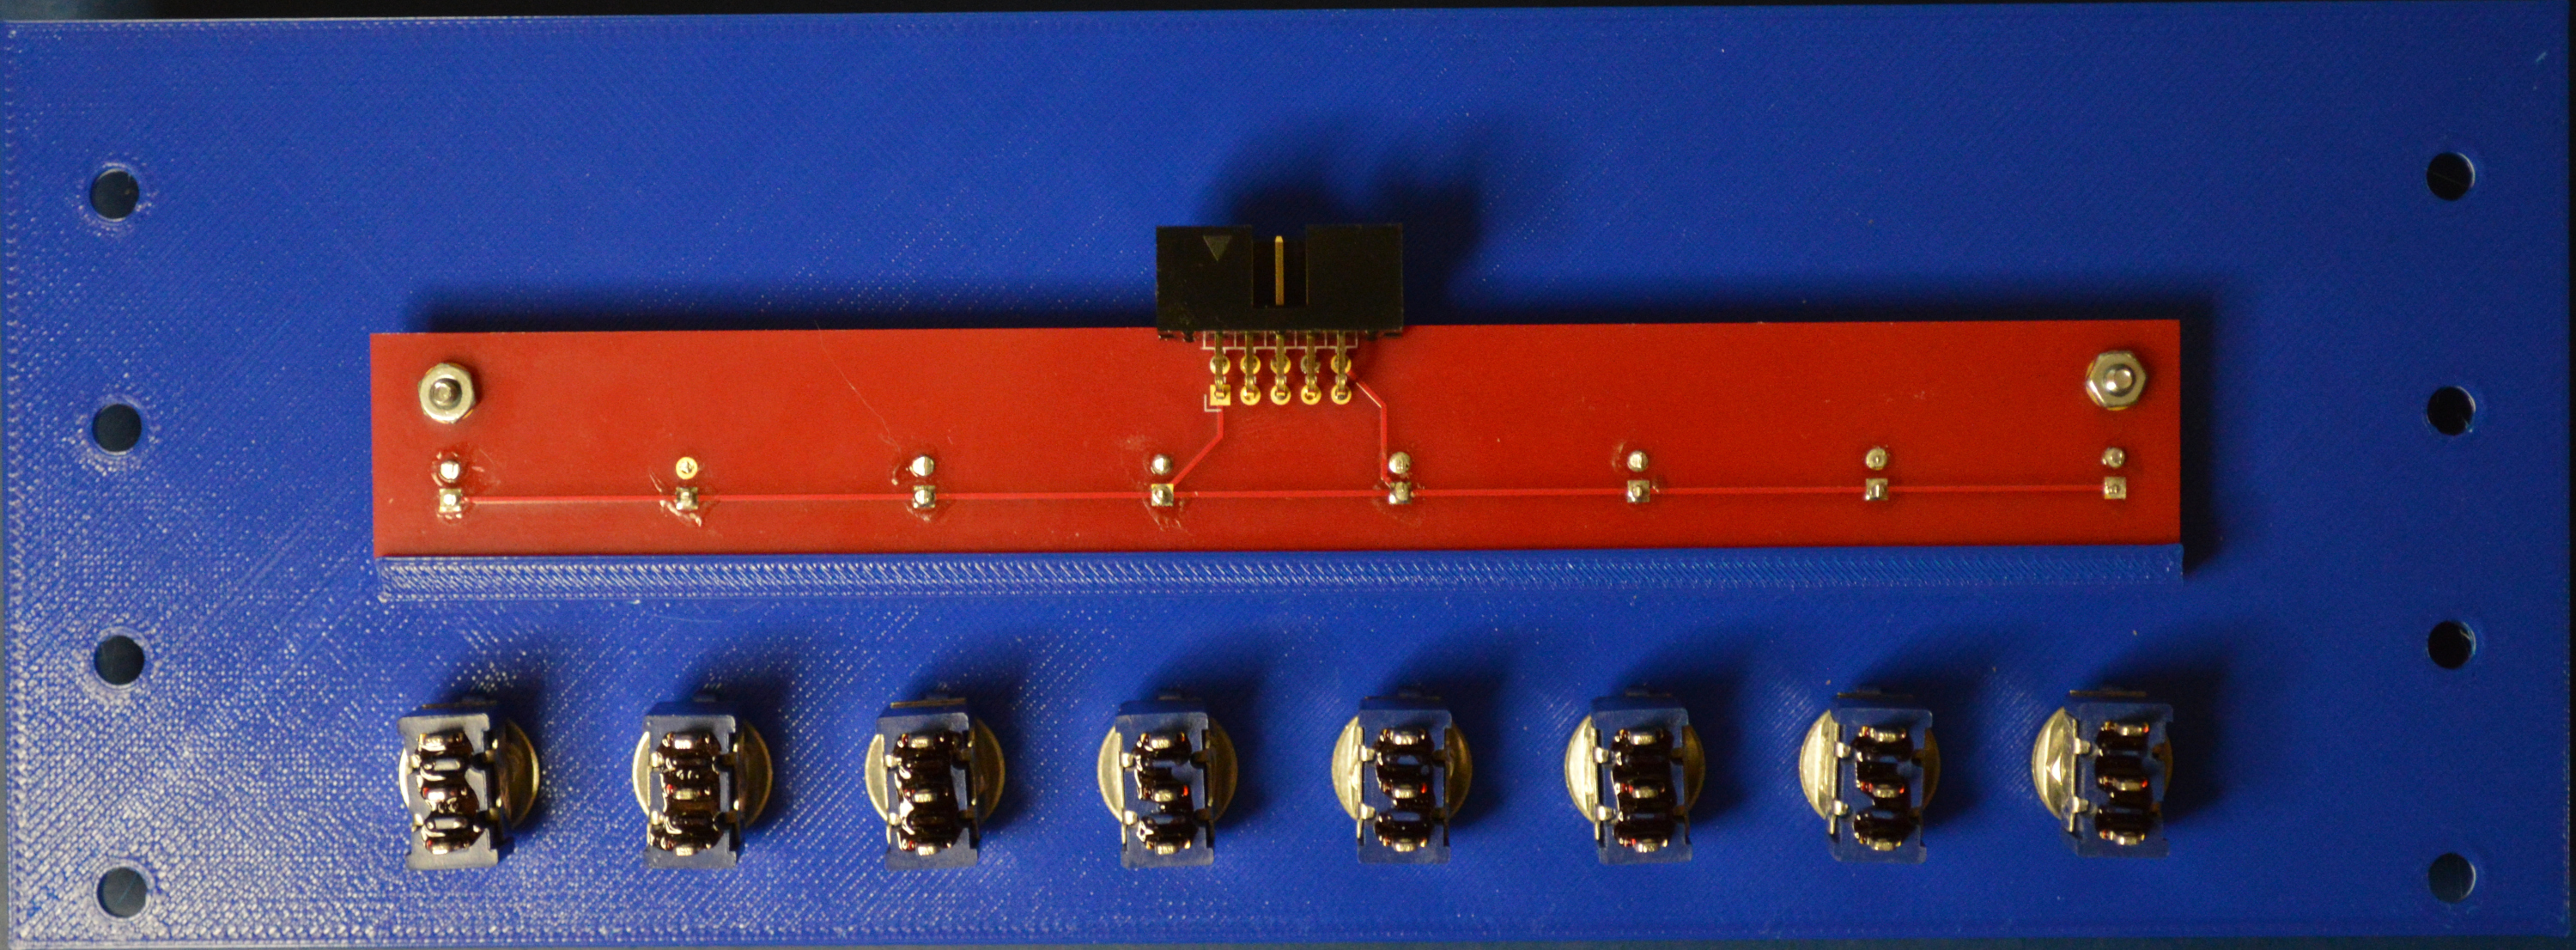
\includegraphics[width=0.9\textwidth]{../Pict/Switch-Installed.jpg}
  \caption{Control Panel Switches Showing Switches Installed}
  \label{fig:SwitchInstalled}
\end{figure}

\begin{figure}[ht!]
  \centering
  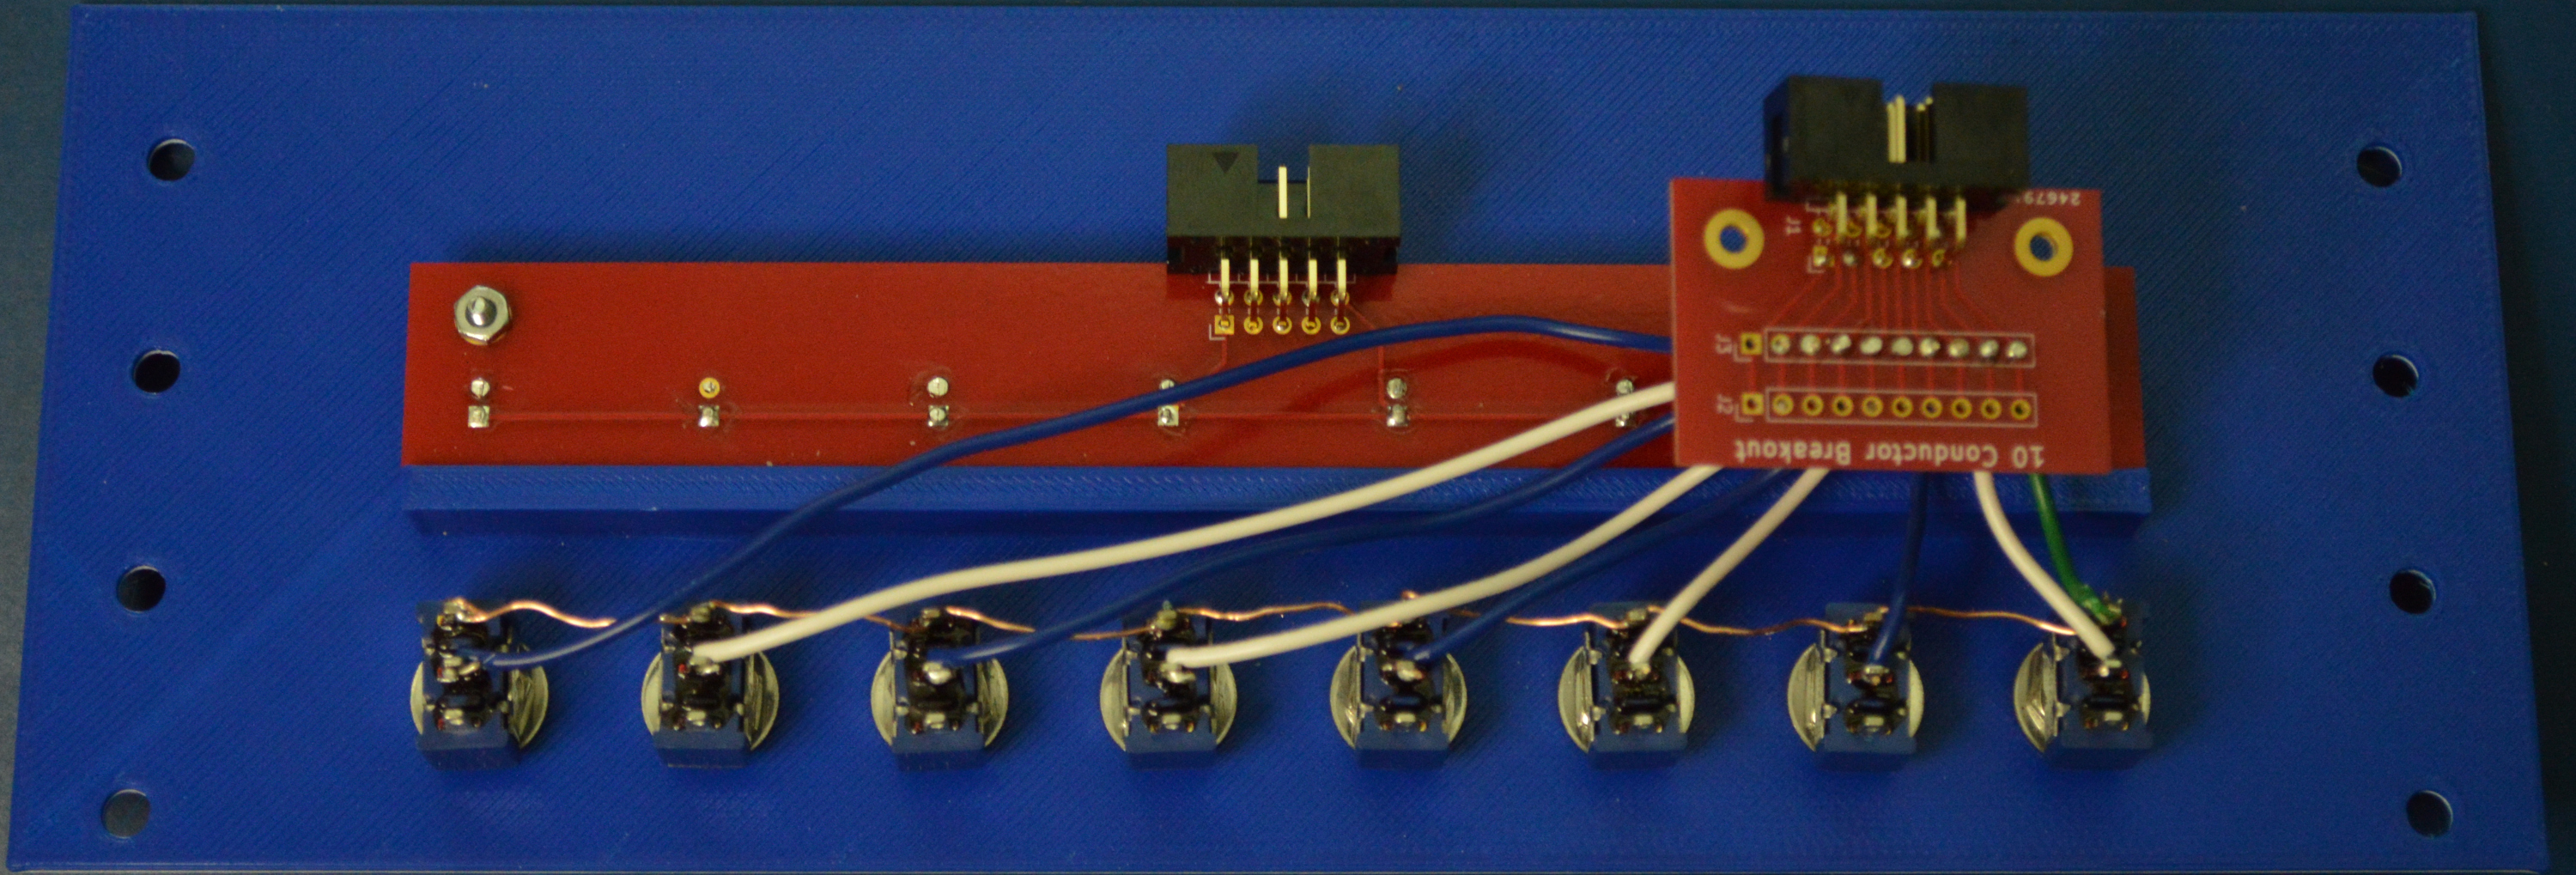
\includegraphics[width=0.9\textwidth]{../Pict/Switch-Wired.jpg}
  \caption{Control Panel Switches Showing Wiring}
  \label{fig:SwitchWired}
\end{figure}

\subsection{I2C Bus Cable}
The I2C Bus Cable is a 10 conductor ribbon cable with crimp-on connectors.  Using this eliminates a lot of tedious soldering that the previous version required.  The pinout for this cable is shown in Table \ref{tbl:I2C-Pins}.

\begin{table}[ht!]
  \caption{I2C Connector Pinout}
  \label{tbl:I2C-Pins}
  \centering
  \begin{tabular}{|r|l|}
    \hline
    Pin & Description\\
    \hline
    1 & No Connection\\
    2 & Ground\\
    3 & No Connection\\
    4 & SDA\\
    5 & No Connection\\
    6 & Vdd\\
    7 & No Connection\\
    8 & SCK\\
    9 & No Connection\\
    10 & Ground\\
    \hline
  \end{tabular}
\end{table}

\section{Power}
You can go with just plugging a USB power adapter into the micro-USB connector on the Raspberry PI, or you can get fancier.  There is a model for a power panel that has cutouts for micro-USB and a USB-B panel mount connectors.  Adafruit offers a number of panel mount USB to various USB adapters.  You can just use one of these.  If you want to get fancier, you can cut open the USB cable and insert the power switch in series with the power conductor.  At this point, you are on your own.  Be careful!

\section{Final Assembly}
Once all of the sub-assemblies are complete, it is time to connect everything together.  It will probably be easiest to start from the bottom and work you way up to the top in assembly.

Since pin 1 of the I/O connectors is on the left side of each connector on the I/O board and LED or switch 1 is on the right side of the panels, the ribbon cables will need a 180$\degree$ twist to them.  When making the I/O cables, put the connector at one end of the cable facing down and the connector at the other end facing up as shown in Figure \ref{fig:GPIOCable}.  On the other hand, the I2C bus cable should have all connectors facing the same direction.

\begin{figure}[ht!]
  \centering
  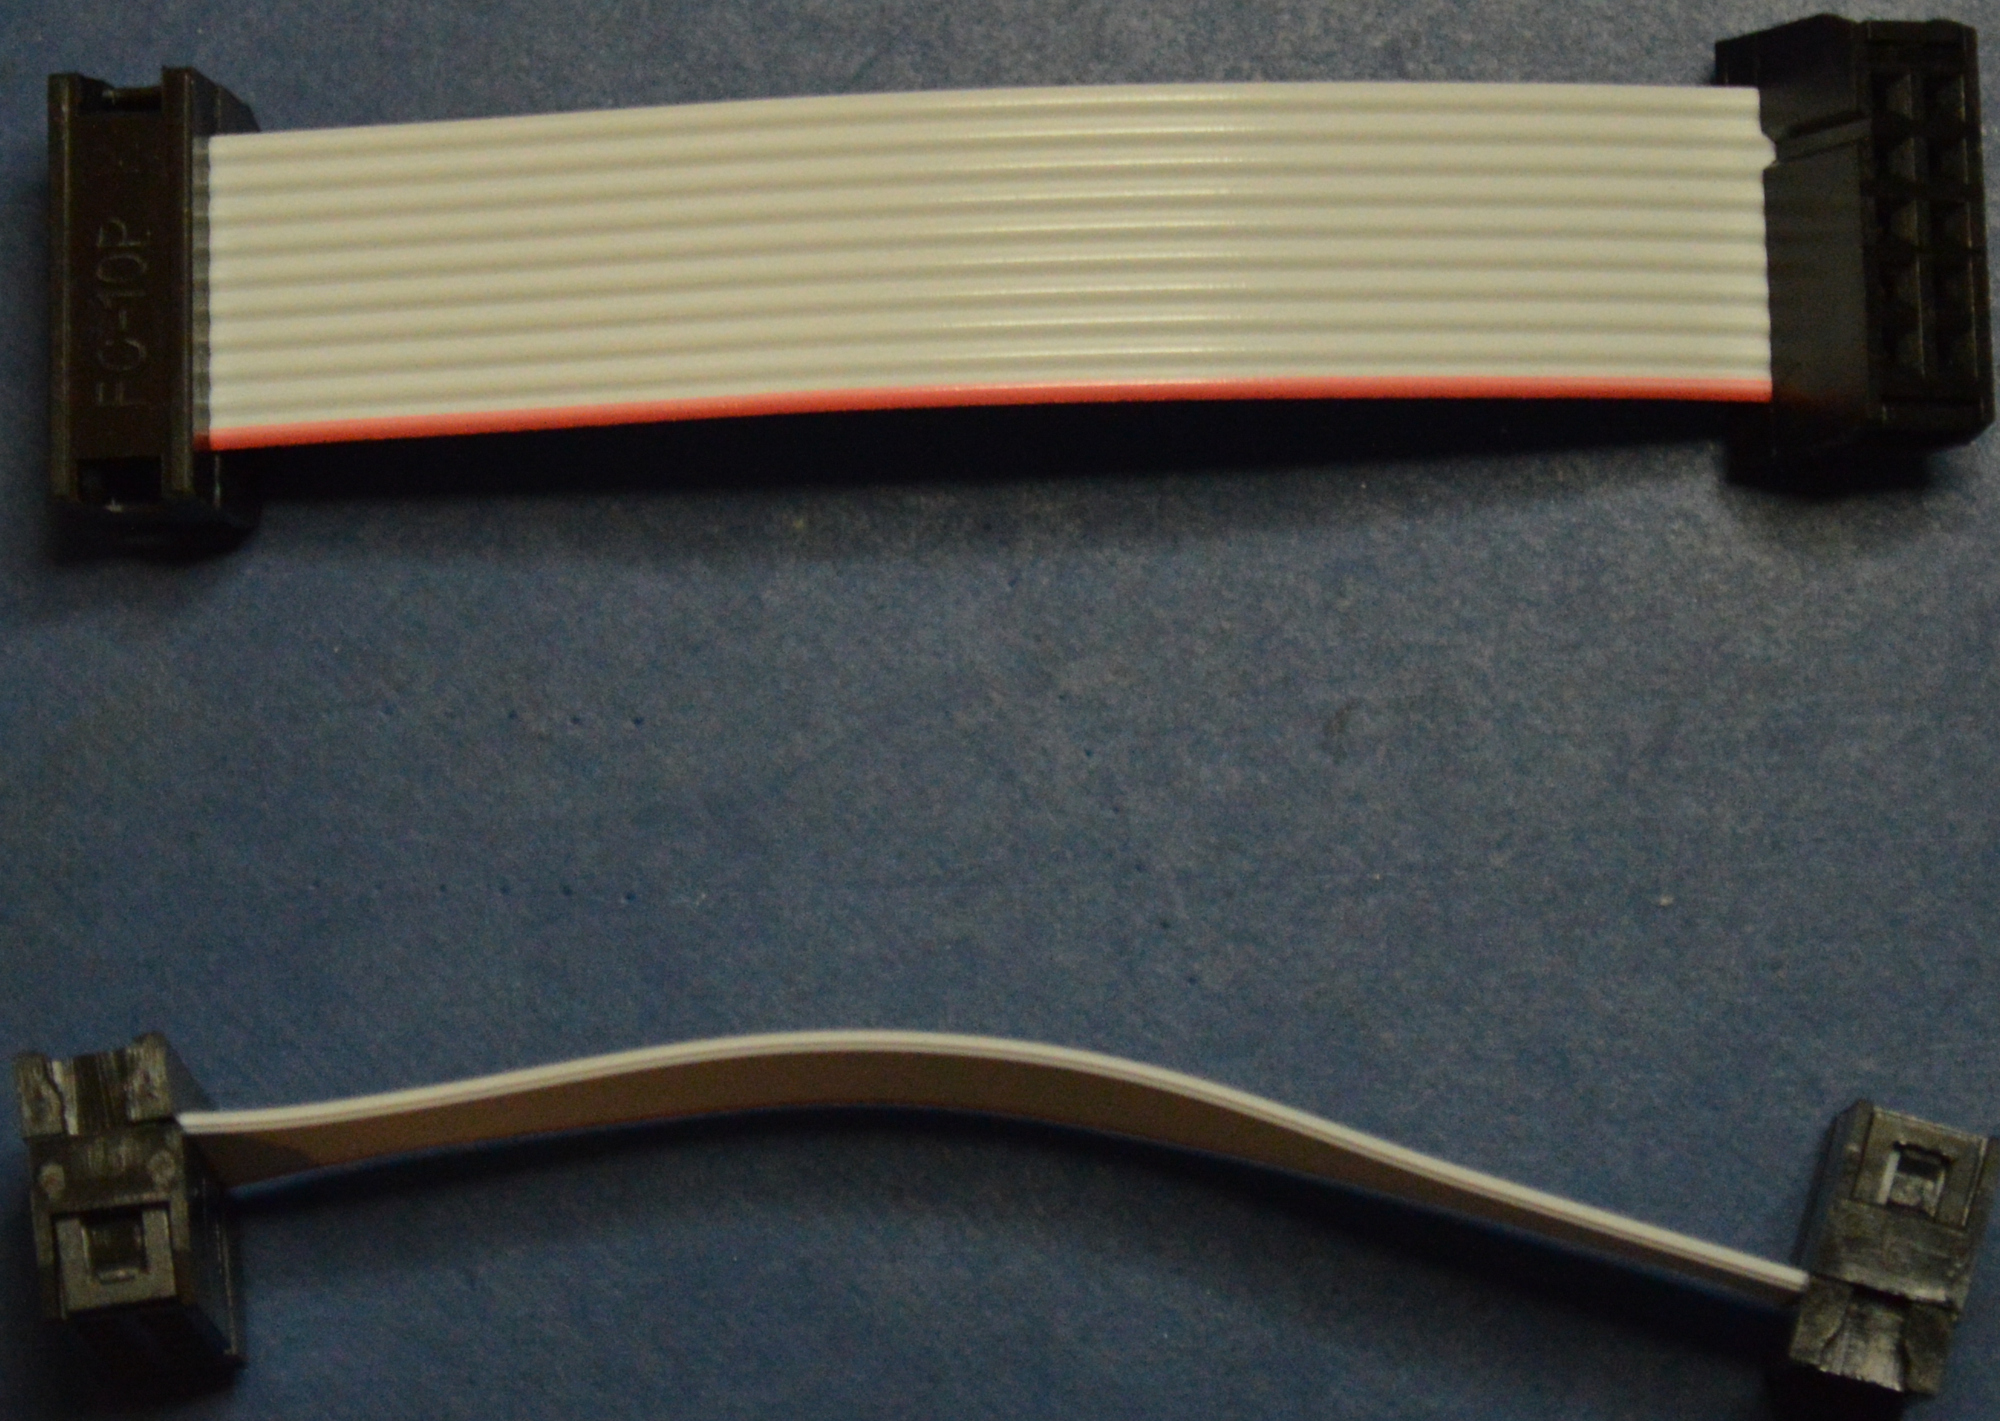
\includegraphics[width=0.9\textwidth]{../Pict/GPIO-Cable.jpg}
  \caption{Example Short GPIO Cables}
  \label{fig:GPIOCable}
\end{figure}

Since there are many options in arranging the various racks, trays, and panels, the lengths of the cables need to be determined on an individual basis.

%----------------------------------------------------------
\chapter{Software}
\section{Overview}
Currently, the software has two main interfaces.  The first is the switches and lights.  The second is a web interface.

\section{Simulation}

\begin{table}
  \caption{Simulations Available}
  \label{tbl:Simulations}
  \centering
  \begin{tabular}{|r|l|}
    \hline
    0 & Copy Switch Values\\
    1 & Count\\
    2 & 16-bit Scan\\
    3 & 16-bit Bounce\\
    4 & Fibonacci Sequence\\
    9 & Count\\
    10 & 32-bit Scan\\
    11 & 32-bit Bounce\\
    12 & Fibonacci Sequence\\
    \hline
    other & Copy Switch Values\\
    \hline
  \end{tabular}
\end{table}

There are a number of ``simulations'' available for testing or display.  The desired simulation can be selected either using the switches, or, if enabled, using the web interface.  The following is a description of the control switches:
\begin{itemize}
  \item The \switch{Power}{Off} switch is intended to be hardwired to the power supply.  There is no program function.
  \item The \position{Exam} switch has no current function.
  \item The \position{Dep} switch is used to select which simulation to run.
  \item The \switch{Addr}{Data} switch has no current function.
  \item The \switch{Auto}{Man} switch enables simulation selection by the web interface when in the \position{Auto} position.
  \item The \switch{Start}{Stop} switch sets all simulation variables to their initial state when moved to the \position{Start} position.  It also must be in the \position{Start} position for the simulation to run.
  \item The \switch{Run}{Pause} switch temporarily pauses a simulation when in the \position{Pause} position.  The simulation continues running without initialization when the switch is moved to the \position{Run} position.
\end{itemize}

Note that for a simulation to run, both the \switch{Start}{Stop} switch must be in the \position{Start} position and the \switch{Run}{Pause} switch must be in the \position{Run} position.

On program initialization, simulation 0 (Copy Switch Values) is selected by default.  To select a different simulation, make sure that either the \switch{Run}{Pause} switch is in the \position{Pause} position or the \switch{Start}{Stop} switch is in the \position{Stop} position.  Then:
\begin{itemize}
  \item Using the \switch{Addr}{Data} switches, select the desired simulation as listed in Table \ref{tbl:Simulations}.
  \item Move the \position{Dep} switch to the \position{Dep} position.  You may need to move it to the unlabeled position first.
  \item Move the \position{Dep} switch to the unlabeled position.
  \item Move the \switch{Run}{Pause} switch to the \position{Run} position.
  \item Move the \switch{Start}{Stop} switch to the \position{Start} position.
\end{itemize}

Unless you wish to reset the simulation values, you should always leave the \switch{Start}{Stop} switch in the \position{Start} position.

\section{Web Server}
The web interface is available on port 31415 (configurable in web.adb).  It uses plain, unencrypted HTTP.

\section{Other Software}
To enhance the experience, you can install some old computer emulation software (such as simh, available at \url{https://github.com/simh/simh}).  Note that this will run completely independent from the lights and switch in this project.

\end{document}

